\documentclass[12pt]{article}\usepackage[]{graphicx}\usepackage[]{color}
% maxwidth is the original width if it is less than linewidth
% otherwise use linewidth (to make sure the graphics do not exceed the margin)
\makeatletter
\def\maxwidth{ %
  \ifdim\Gin@nat@width>\linewidth
    \linewidth
  \else
    \Gin@nat@width
  \fi
}
\makeatother

\definecolor{fgcolor}{rgb}{0.345, 0.345, 0.345}
\newcommand{\hlnum}[1]{\textcolor[rgb]{0.686,0.059,0.569}{#1}}%
\newcommand{\hlstr}[1]{\textcolor[rgb]{0.192,0.494,0.8}{#1}}%
\newcommand{\hlcom}[1]{\textcolor[rgb]{0.678,0.584,0.686}{\textit{#1}}}%
\newcommand{\hlopt}[1]{\textcolor[rgb]{0,0,0}{#1}}%
\newcommand{\hlstd}[1]{\textcolor[rgb]{0.345,0.345,0.345}{#1}}%
\newcommand{\hlkwa}[1]{\textcolor[rgb]{0.161,0.373,0.58}{\textbf{#1}}}%
\newcommand{\hlkwb}[1]{\textcolor[rgb]{0.69,0.353,0.396}{#1}}%
\newcommand{\hlkwc}[1]{\textcolor[rgb]{0.333,0.667,0.333}{#1}}%
\newcommand{\hlkwd}[1]{\textcolor[rgb]{0.737,0.353,0.396}{\textbf{#1}}}%
\let\hlipl\hlkwb

\usepackage{framed}
\makeatletter
\newenvironment{kframe}{%
 \def\at@end@of@kframe{}%
 \ifinner\ifhmode%
  \def\at@end@of@kframe{\end{minipage}}%
  \begin{minipage}{\columnwidth}%
 \fi\fi%
 \def\FrameCommand##1{\hskip\@totalleftmargin \hskip-\fboxsep
 \colorbox{shadecolor}{##1}\hskip-\fboxsep
     % There is no \\@totalrightmargin, so:
     \hskip-\linewidth \hskip-\@totalleftmargin \hskip\columnwidth}%
 \MakeFramed {\advance\hsize-\width
   \@totalleftmargin\z@ \linewidth\hsize
   \@setminipage}}%
 {\par\unskip\endMakeFramed%
 \at@end@of@kframe}
\makeatother

\definecolor{shadecolor}{rgb}{.97, .97, .97}
\definecolor{messagecolor}{rgb}{0, 0, 0}
\definecolor{warningcolor}{rgb}{1, 0, 1}
\definecolor{errorcolor}{rgb}{1, 0, 0}
\newenvironment{knitrout}{}{} % an empty environment to be redefined in TeX

\usepackage{alltt}\usepackage[]{graphicx}\usepackage[]{color}
%% maxwidth is the original width if it is less than linewidth
%% otherwise use linewidth (to make sure the graphics do not exceed the margin)
\makeatletter
\def\maxwidth{ %
  \ifdim\Gin@nat@width>\linewidth
    \linewidth
  \else
    \Gin@nat@width
  \fi
}
\makeatother

\definecolor{fgcolor}{rgb}{0.345, 0.345, 0.345}
\newcommand{\hlnum}[1]{\textcolor[rgb]{0.686,0.059,0.569}{#1}}%
\newcommand{\hlstr}[1]{\textcolor[rgb]{0.192,0.494,0.8}{#1}}%
\newcommand{\hlcom}[1]{\textcolor[rgb]{0.678,0.584,0.686}{\textit{#1}}}%
\newcommand{\hlopt}[1]{\textcolor[rgb]{0,0,0}{#1}}%
\newcommand{\hlstd}[1]{\textcolor[rgb]{0.345,0.345,0.345}{#1}}%
\newcommand{\hlkwa}[1]{\textcolor[rgb]{0.161,0.373,0.58}{\textbf{#1}}}%
\newcommand{\hlkwb}[1]{\textcolor[rgb]{0.69,0.353,0.396}{#1}}%
\newcommand{\hlkwc}[1]{\textcolor[rgb]{0.333,0.667,0.333}{#1}}%
\newcommand{\hlkwd}[1]{\textcolor[rgb]{0.737,0.353,0.396}{\textbf{#1}}}%
\let\hlipl\hlkwb

\usepackage{framed}
\makeatletter
\newenvironment{kframe}{%
 \def\at@end@of@kframe{}%
 \ifinner\ifhmode%
  \def\at@end@of@kframe{\end{minipage}}%
  \begin{minipage}{\columnwidth}%
 \fi\fi%
 \def\FrameCommand##1{\hskip\@totalleftmargin \hskip-\fboxsep
 \colorbox{shadecolor}{##1}\hskip-\fboxsep
     % There is no \\@totalrightmargin, so:
     \hskip-\linewidth \hskip-\@totalleftmargin \hskip\columnwidth}%
 \MakeFramed {\advance\hsize-\width
   \@totalleftmargin\z@ \linewidth\hsize
   \@setminipage}}%
 {\par\unskip\endMakeFramed%
 \at@end@of@kframe}
\makeatother

\definecolor{shadecolor}{rgb}{.97, .97, .97}
\definecolor{messagecolor}{rgb}{0, 0, 0}
\definecolor{warningcolor}{rgb}{1, 0, 1}
\definecolor{errorcolor}{rgb}{1, 0, 0}
\newenvironment{knitrout}{}{} % an empty environment to be redefined in TeX

\usepackage{alltt}
\usepackage{booktabs}
\usepackage[english]{babel}
\usepackage[utf8]{inputenc}
\usepackage{amsmath}
\usepackage{bm}
\usepackage{graphicx}
\usepackage{cite}
\def\citepunct{; \penalty\citepunctpenalty}
\usepackage{url}
\usepackage{soul}
\usepackage{caption}
\usepackage{setspace}
\IfFileExists{upquote.sty}{\usepackage{upquote}}{}
\usepackage{listings}
\usepackage{amsthm}
\usepackage[linewidth=1pt]{mdframed}
\usepackage{lipsum}
%\usepackage{natbib}
%\usepackage[round]{natbib} 
\usepackage{apalike}
\lstset{
	language=R,
	basicstyle=\ttfamily
}
\usepackage{epsfig} % eps graphics
%authoryear,open={(},close={)}}
\IfFileExists{upquote.sty}{\usepackage{upquote}}{}
\begin{document}




\begin{titlepage}

\newcommand{\HRule}{\rule{\linewidth}{0.5mm}} % Defines a new command for the horizontal lines, change thickness here

\center % Center everything on the page
 
%----------------------------------------------------------------------------------------
%   HEADING SECTIONS
%----------------------------------------------------------------------------------------

\textsc{\LARGE Montana State University}\\[0.5cm] % Name of your university/college
\textsc{\Large Department of Mathematical Sciences}\\[0.5cm] % Major heading such as course name
\textsc{\large Writing Project}\\[.75cm] % Minor heading such as course title

%----------------------------------------------------------------------------------------
%   TITLE SECTION
%----------------------------------------------------------------------------------------

\HRule \\[0.4cm]
{ \huge \bfseries TITLE }\\[0.4cm] % Title of document
\HRule \\[1.5cm]
 
%----------------------------------------------------------------------------------------
%   AUTHOR SECTION
%----------------------------------------------------------------------------------------

\begin{minipage}{0.4\textwidth}
\begin{flushleft} 
\large
\emph{Author:} \\
\textsc{Meaghan Winder} \\
\end{flushleft}
\end{minipage}
~
\begin{minipage}{0.4\textwidth}
\begin{flushright} 
\large
\emph{Supervisor:} \\
\textsc{Dr. Andrew Hoegh} 
\end{flushright}
\end{minipage}\\[1.5cm]

%----------------------------------------------------------------------------------------
%   DATE SECTION
%----------------------------------------------------------------------------------------

{\large Spring 2020}\\[1.5cm] % Date, change the \today to a set date if you want to be precise

%----------------------------------------------------------------------------------------
%   LOGO SECTION
%----------------------------------------------------------------------------------------


\includegraphics[width=5cm]{msulogo} % Include a department/university logo - this will require the graphicx package
 
%----------------------------------------------------------------------------------------

A writing project submitted in partial fulfillment\\
of the requirements for the degree\\[.25in]
Master's of Science in Statistics

\vfill % Fill the rest of the page with whitespace

\end{titlepage}

\begin{titlepage}
\null
\begin{center}
{\bf\huge APPROVAL}\\[1.0 in]
of a writing project submitted by\\[.25 in]
Meaghan Winder \\[0.5 in]
\end{center}

\noindent
This writing project has been read by the writing project advisor and
has been found to be satisfactory regarding content, English usage,
format, citations, bibliographic style, and consistency, and is ready
for submission to the Statistics Faculty.

\vspace{.3in}
\begin{center}
\begin{tabular}{ll}
\rule{2.75in}{.03in} & \rule{2.75in}{.03in} \\
Date& Andrew Hoegh \\
& Writing Project Advisor \\
\end{tabular}
\end{center}

\vspace{1cm}

\begin{center}
\begin{tabular}{ll}
\rule{2.75in}{.03in} & \rule{2.75in}{.03in} \\
Date& Mark C. Greenwood \\
& Writing Projects Coordinator \\
\end{tabular}
\end{center}

\end{titlepage}

\newpage
\tableofcontents
\newpage

\begin{abstract}
\noindent abstract text here 
\end{abstract}

\doublespacing

\section{Introduction}

In early 2020, the City of Austin, Texas approved the spending of four million dollars over the next five years in an attempt to remove zebra mussels from the city's source of drinking water with a liquid copper sulfate pentahydrate released into the water intake pipes \cite{CBS:Austin}. This is one of many pursuits to remove dreissenid mussels\footnote{Zebra mussels (\textit{Dreissena polymorpha}) and quagga mussels (\textit{Dreissena rostriformis bugensis}) collectively.} from water bodies across the United States, and four million dollars is merely a small fraction of what is spent annually on control and mitigation efforts.

Zebra mussels are native to the Caspian and Black Seas, but have become widespread in both Europe and the United States; they were discovered in the Great Lakes in the late 1980s and have since spread rapidly across the continental U.S. The United States National Park Service stated that ``[o]nce a population of zebra mussels has become established in a water body, there is very little to be done to remove them. Prevention, therefore, is the best way to keep a water body clean of zebra mussels'' \cite{NPS}; hence, early detection of invasive species, such as dreissenid mussels, has become a priority in order for organizations to plan, budget, and install necessary technologies before colonization has occurred \cite{Holser:body}. 

\begin{figure}[]
	\centering
	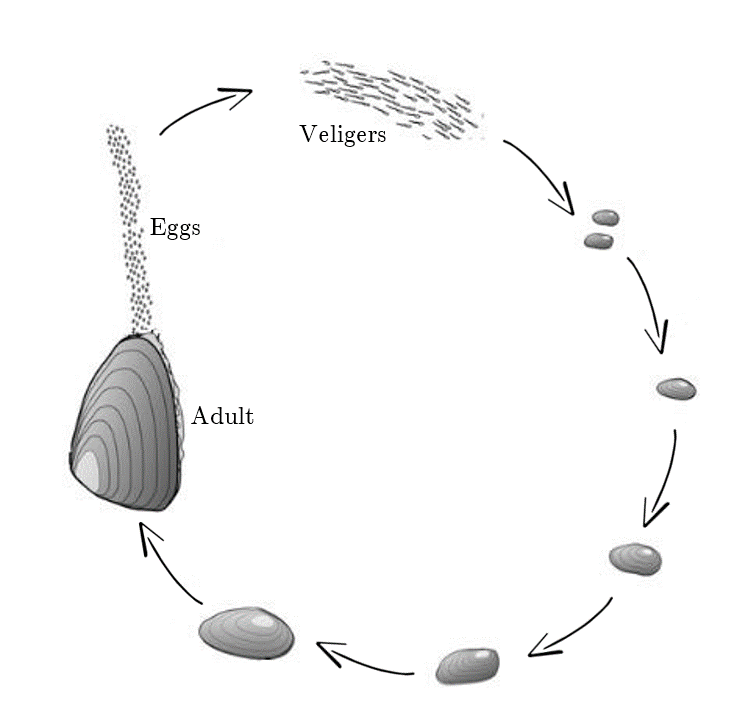
\includegraphics[scale = 0.7]{images/lifecycle}
	\caption{A diagram depicting the life cycle of dreissenid mussels.}
	\label{fig:lifecycle}
\end{figure}

Zebra mussels live between two and five years; they start as microscopic veligers but mature to thumbnail sized adults; they begin reproduction at two years of age, after which, females can release up to one million eggs per year \cite{NPS}. A diagram depicting the life cycle of dreissenid mussels is shown in Figure \ref{fig:lifecycle}. Dreissenid mussel veligers free-swim in the water; often, they travel to uninfested waters on boats or through other aquatic recreational activities, however, sometimes they are moved by nature and travel downstream to uninfested waters. Adult dreissenids attach and colonize hard surfaces in the water, this process of accumulation of adult zebra mussels on rocks, native mussels, docks, boats, or other hard surfaces is referred to as ``biofouling,'' and objects that are in the water for long periods of time become difficult and costly to clean.

Once a water body is colonized by adult dreissenid mussels, water supply and delivery facilities, water recreation sites, and other water dependent economies in that body of water become much more expensive to maintain and operate \cite{BOR}. For example, after dreissenid mussels were detected in Montana's Tiber Reservoir in 2016, with suspected detections in Canyon Ferry Reservoir as well, the state of Montana highlighted the economic impacts that a full dreissenid mussel colonization could have on the state; in January 2019, the Montana Department of Natural Resources and Conservation published a report titled \textit{Enumeration of Potential Economic Costs of Dreissenid Mussels Infestation in Montana}. The report states that if dreissenid mussels were to infest every lake and river in Montana, it could cost the state more than 230 million dollars annually in mitigation costs, as well as lost revenue \cite{MT}. 

Dreissenid infestations result not only in economic impacts, but in environmental ones as well. Dreissenid mussels are filter feeders and siphon plankton from the water, which can lead to changes the water body ecosystem by increasing water clarity; a single adult dreissenid can filter about a liter of water per day, which reduces the availability of algae for native mussels and bottom feeding fish \cite{BOR}. Additionally, ``biofouling'' can prevent native mussels from moving, feeding, reproducing, or regulating the water system. Several actions, such as the 2017 initiative, \textit{Safeguarding the West from Invasive Species}, by the Department of the Interior, have been taken to protect water bodies in the western United States from the economic and ecological threats posed by the invasive dreissenid mussels. Early detection of dreissenid mussels can reduce the economic and ecological repercussions of dreissenid infestations, however there are issues with the available early detection methods. 

The established standard for early detection of dreissenids in the western United States is plankton tow sampling for mussel veligers. Using a fine mesh net, water and debris are collected at multiple sampling sites within each water body; the debris from each net collected at the same sampling site on the same day is aggregated and examined, using cross-polarized light microscopy, for the free-swimming veligers. Following the microscopic examination, positive species identification is confirmed using polymerase chain reaction (PCR) chemistry. This early detection method requires a breeding population, so is limited to the weeks immediately following a spawning event \cite{Nichols}; spawning begins at water temperatures above 10$^\circ$C for quagga mussels and above 12$^\circ$C for zebra mussels \cite{McMahon, Mills}. This suggests that veliger availability in northern latitude water bodies is typically limited to warmer months \cite{Sepulveda:eDNA}.

An alternative method, growing in popularity, for detection of rare, endangered, or invasive species, is environmental DNA (eDNA) surveys \cite{Schmelzle}. Environmental DNA methods can detect DNA diffused by the target species in water sampled from a water body. Multiple water samples are collected from each sampling site within a lake, the samples are then analyzed using one of several different types of PCR chemistry. Sepulveda, Amberg, and Hanson (2019) suggest the use of eDNA surveys may widen the seasonal sampling window of plankton tow methods, since eDNA does not rely on a breeding population. Environmental DNA surveys are more time and cost effective than traditional sampling methods for species of low abundance \cite{Rees}. However, a positive eDNA result does not necessarily indicate that the target species is present or alive at the site; positive eDNA results can be obtained from ``a failed introduction, from external sources, or from field contamination, rather than fresh DNA from mussel colonization'' \cite{Sepulveda:eDNA}. One criticism of the detection of dreissenid mussels using eDNA is there is a possibility of obtaining false-positive results; since control efforts for invasive species are costly, there is some hesitation in using eDNA surveys as the sole decision-making tool for the management of dreissenid mussels. When the two early detection methods result in conflicting answers, decision making can be even more complicated, since a positive eDNA result suggests only that the DNA of the target species is present, regardless of whether the species is alive or even present at all, but when veligers are detected, positive eDNA results indicate a potential colonization, which is useful to managers \cite{Holser:body}. 

Occupancy models allow the occurrence of a species to be accurately estimated, even when the species is imperfectly detected. For both the plankton tow and eDNA surveys, there is a non-zero probability of a false negative result. Since plankton tow survey methods are restricted to capturing only mussel veligers, dreissenid mussels can be present in the lake and not be captured in the plankton tow nets at one or more of the sampling sites, either because the veligers are missed with the nets or because there are no free-swimming veligers available in the water; even if the veligers are captured in the net, there is a possibility that they are not detected using cross-polarized light microscopy. Similarly for eDNA methods, dreissenid mussels could be present in the lake, but their DNA could be missed in one or more of the samples from each of the sampling sites; even if dreissenid mussel DNA is present in the sample, it could be missed in the PCR replicate. Replication in the survey design can help researchers learn about the detection probabilities for each of the early detection methods. 

\hl{\textit{Some research question about the detection probability.}} Furthermore, sampling recommendations such as how many samples to take at low concentration sites and how many samples are necessary to ensure a high probabilty of at least one detection at the sites with low concentrations are of interest. \hl{\textit{A few sentences here about the structure of the rest of the paper.}}

\section{Data}



The eDNA data were collected during the spring, summer, and fall of 2019 as part of a study on the detection of dreissenid mussels and Asian clams in northeastern lakes using environmental DNA. There were six lakes surveyed across Maine, New Hampshire, New York, and Vermont; each lake was sampled for dreissenid mussels, Asian clams, or both. The data available are from three of the lakes sampled for dreissenid mussels. There are multiple sites within each lake, from each, five one-liter water samples were collected. Most sites were visited on more than one day throughout the course of the study. Each of the samples were analyzed using a DNA amplification technique, known as digital droplet PCR (ddPCR), on a Biorad Digital Droplet PCR system using dreissenid mussel assays. This PCR technique divides the sample aliquot into micro droplets to be analyzed separately. A field blank of clean lab water accompanied the set of five samples from each site on a given day to ensure no cross contamination in the lab. Droplet replications for dreissenid mussel DNA were negative for all field blank samples; these samples were removed from the data set. 

The lakes are coded ``BOM,'' ``LG,'' and ``MG,'' and these names will be used throughout. There are three sites in lake BOM (BOM1, BOM2, BOM3), each of which was sampled five times on three different days (May 28, July 8, and October 21), for a total of 15 samples per site and 45 total samples from lake BOM. There are five sites in lake LG; the first three sites (LG1, LG2, LG3) were sampled five times on both May 28 and July 8, and the final two sites (LG4, LG5) were each sampled five times on September 25, for a total of 40 samples from lake LG. There were originally five sites in lake MG, but one (MG2) was inaccessible on the study day, so there are data for four sites in lake MG (MG1, MG3, MG4, MG5), each of which was sampled five times on August 23, for a total of 20 samples from lake MG. In all, there are twelve sites and 105 samples. Each of the samples were divided into thousands of droplets for ddPCR analysis. Figure \ref{fig:eDNA_diagram} illustrates the hierarchical structure of the eDNA data within a lake. Ten sample rows of the data set are displayed in Table \ref{tab:eDNA_data}, where ``Positive Droplets'' is the number of droplets where dreissenid mussel DNA was amplified and ``Concentration'' is the number of copies of target DNA per microliter of extraction (copies/$\mu$L)?}}. Water temperatures ($^\circ$C) were also recorded at each site on each study day, with the exception of temperatures at sites in lake BOM on October 21. 

\begin{figure}[]
	\centering
	
\includegraphics[scale = 0.7]{images/eDNA}
	\caption{A diagram displaying the hierarchical structure of the eDNA data.}
	\label{fig:eDNA_diagram}
\end{figure}

\begin{knitrout}
\definecolor{shadecolor}{rgb}{0.969, 0.969, 0.969}\color{fgcolor}\begin{table}[!h]

\caption{\label{tab:eDNA_table}\label{tab:eDNA_data}
             10 sample rows of the eDNA data.}
\centering
\resizebox{\linewidth}{!}{
\begin{tabular}[t]{ccccccc}
\toprule
Lake & Site & Sample & Date & Water Temperature & Concentration & Positive Droplets\\
\midrule
BOM & BOM1 & BOM1w0528195 & 5/28/2019 & 11.0 & 8.51 & 60\\
BOM & BOM1 & BOM1w0708194 & 7/8/2019 & 25.5 & 0.81 & 7\\
BOM & BOM2 & BOM2w1021191 & 10/21/2019 & NA & 1.14 & 8\\
BOM & BOM3 & BOM3w0528193 & 5/28/2019 & 6.0 & 178.72 & 1154\\
BOM & BOM3 & BOM3w0708193 & 7/8/2019 & 24.5 & 175.99 & 1388\\
BOM & BOM3 & BOM3w1021191 & 10/21/2019 & NA & 2.04 & 13\\
LG & LG1 & LG1w0528194 & 5/28/2019 & 12.0 & 0.00 & 0\\
LG & LG2 & LG2w0708194 & 7/8/2019 & 23.0 & 0.00 & 0\\
LG & LG2 & LG2w0708195 & 7/8/2019 & 23.0 & 0.00 & 0\\
MG & MG5 & MG5w082319D & 8/23/2019 & 18.3 & 0.00 & 0\\
\bottomrule
\end{tabular}}
\end{table}


\end{knitrout}



The number of positive droplets per sample range between 0 and 3331 for lake BOM, between 0 and 3 for lake LG, and between 0 and 2 for lake MG. Based on Figure \ref{fig:eDNA_droplets} it is clear that the samples taken on May 28 and July 8 from sites BOM2 and BOM3 tend to have the highest numbers of positive droplets, while the samples at the remaining sites across their respective sampling dates, and the samples taken on October 21 at sites BOM2 and BOM3 all have numbers positive droplets near 0. It is noted that samples with fewer than three positive droplets should be treated with caution, as they have potential to be false positives. This is immediately noticeable in lakes LG and MG, as all the values of positive droplets per sample are low for these two lakes. Of the 40 samples from lake LG, 38 of them resulted in no positive droplets, and the remaining two samples resulted in two or three positive droplets per sample. Similarly for lake MG, 16 of the 20 samples resulted in no positive droplets, and the remaining samples resulted in one or two positive droplets per sample. While larger numbers of positive droplets were observed in samples from lake BOM, there are still three samples which resulted in some, but fewer than three, positive droplets. To limit the possibility of false positive samples for these analyses, to be considered a positive sample, the recommended threshold of three or more positive droplets will be used. The top plot in Figure \ref{fig:eDNA_sample} displays the proportion of positive samples by site if all samples with positive droplets are treated as positive samples, and the bottom plot displays the proportion of positive samples by site using the above threshold to limit the positive sites to those with three or more positive droplets. Figure \ref{fig:eDNA_sample} can be used to visualize the changes in the proportion of positive samples from each site when the threshold is used. The use of the threshold changes the proportion of positive samples in six of the twelve sites; the proportion of positive samples are: 0.5333 for site BOM1, 0.9333 for site BOM2, 0.8666 for lake BOM3, 0.0000 for sites LG1, LG2, LG4, and LG5, 0.1000 for site LG2,  and finally 0.0000 for all sites in lake MG.

\begin{figure}[]
\begin{knitrout}
\definecolor{shadecolor}{rgb}{0.969, 0.969, 0.969}\color{fgcolor}

{\centering 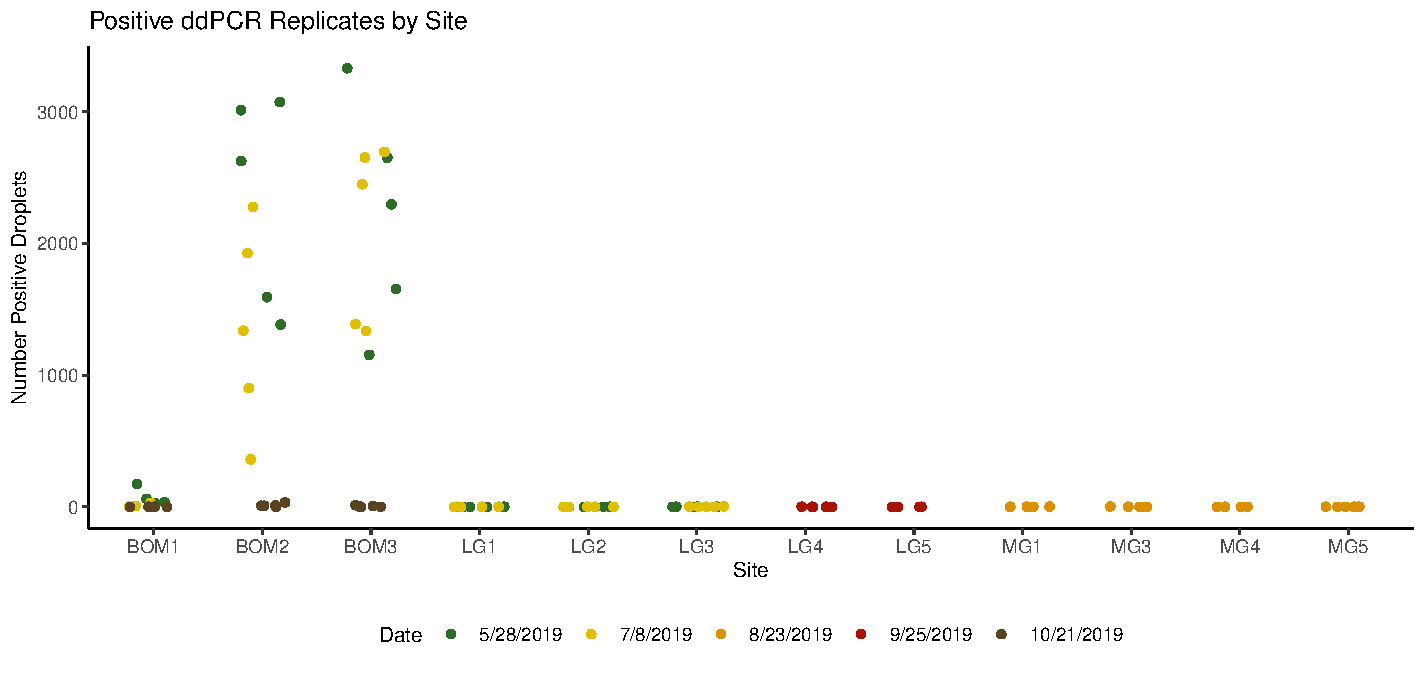
\includegraphics[width=\maxwidth]{figure/eDNA_visualization_droplets-1} 

}



\end{knitrout}
\caption{A plot of the positive droplets from each sample by site, colored by the date on which the sample was taken.}
\label{fig:eDNA_droplets}
\end{figure}



\begin{figure}[]
\begin{knitrout}
\definecolor{shadecolor}{rgb}{0.969, 0.969, 0.969}\color{fgcolor}

{\centering 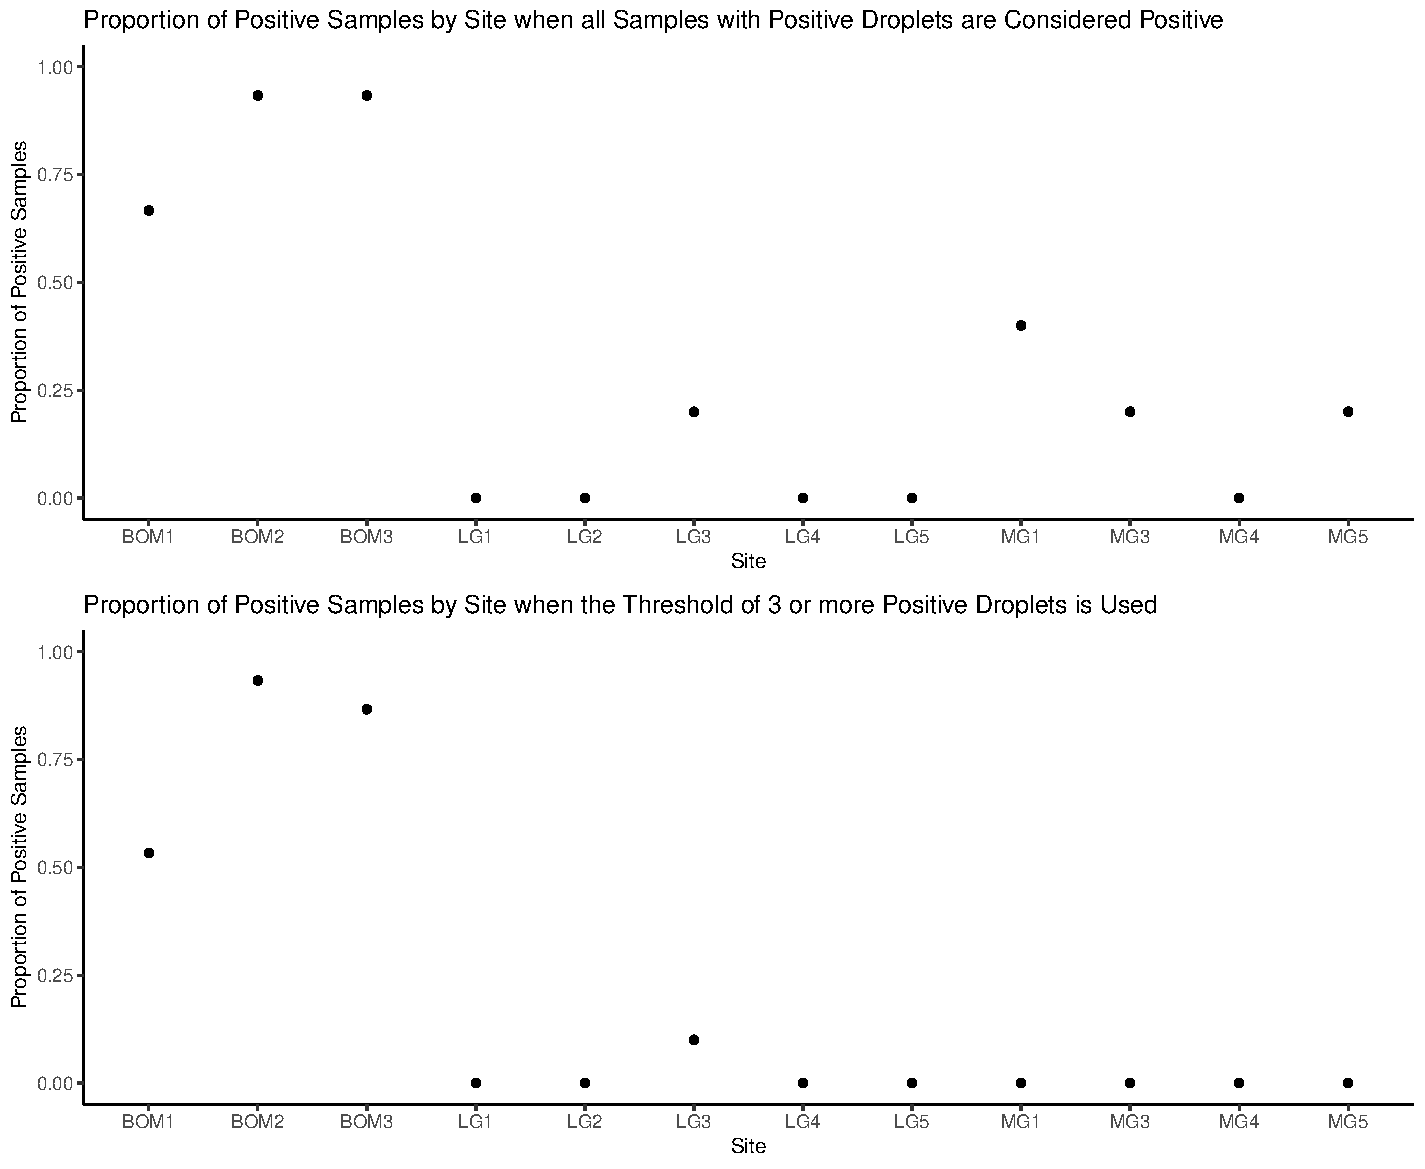
\includegraphics[width=\maxwidth]{figure/eDNA_visualization_sample-1} 

}



\end{knitrout}
\caption{A plot of the proportion of positive droplets by site if all samples with any positive droplets are treated as positive detections (top), and a plot of the proportion by site if samples with fewer than three positive droplets are treated as negative (bottom).}
\label{fig:eDNA_sample}
\end{figure}

The concentrations in the study range between 0.00 and 733.80 copies/$\mu$L. Based on the top plot in Figure \ref{fig:eDNA_concentration}, it is clear that the sites with the highest concenrations occur in samples from sites BOM2 and BOM3, with average concentrations of 206 and 235 copies/$\mu$L  in each of the respective sites. Sites LG1, LG2, LG4, LG5, and MG4 all have average concentrations of 0 copies /$\mu$L. The samples from the remaining sites tend to have low, but non-zero concenrations; the bottom plot in Figure \ref{fig:eDNA_concentration} displays the samples by site for non-zero concentrations below 10 copies/$\mu$L.  



\begin{figure}[]
\begin{knitrout}
\definecolor{shadecolor}{rgb}{0.969, 0.969, 0.969}\color{fgcolor}

{\centering 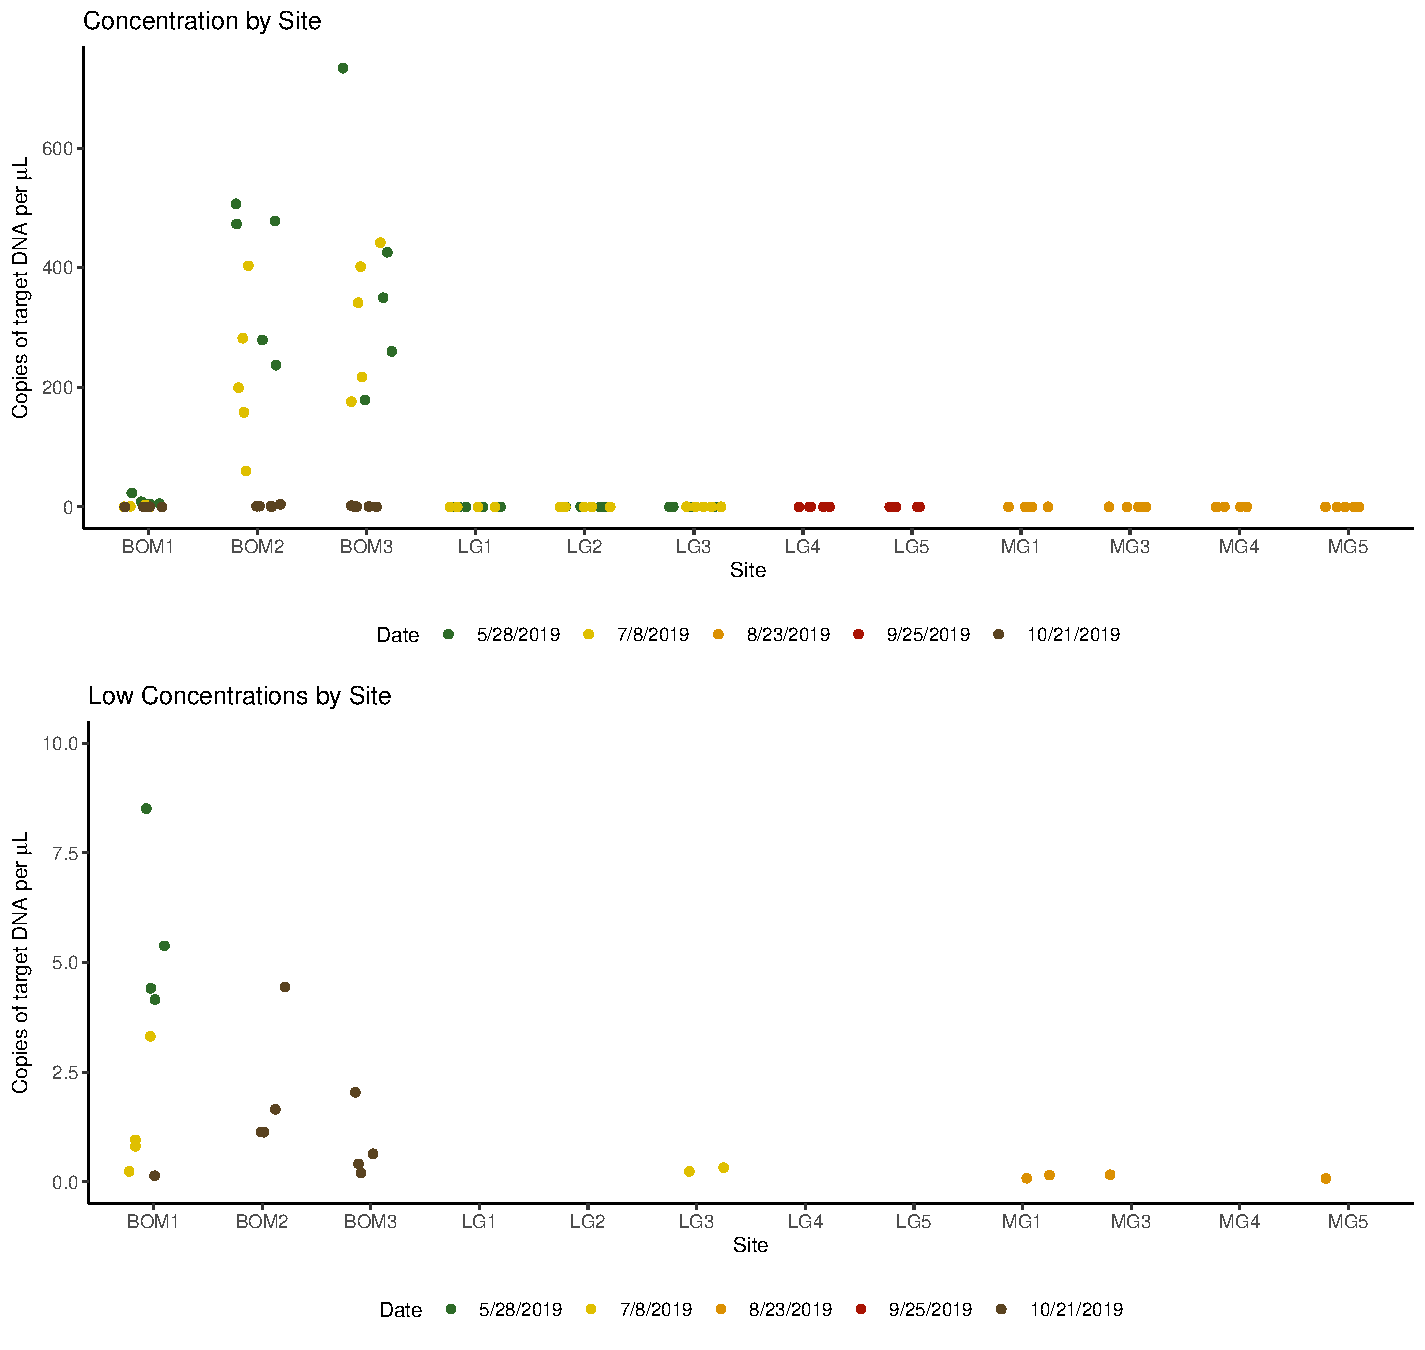
\includegraphics[width=\maxwidth]{figure/eDNA_visualization_concentration-1} 

}



\end{knitrout}
\caption{A plot displaying the number of copies of target DNA per $\mu$L per sample by site (top), and a plot displaying the number of copies of target DNA per $\mu$L for samples with low, but non-zero, concentrations.}
\label{fig:eDNA_concentration}
\end{figure}

Water temperature could play a role in the availability of dreissenid mussel eDNA in the water, or the probability that the DNA is able to be detected using ddPCR. The water temperatures observed in lake BOM range from 6$^\circ$C to 25.5$^\circ$C, but temperatures were not recorded at any of the sites in lake BOM on October 21. The temperatures from a USGS gauge at a nearby lake, were positively adjusted by 2$^\circ$C to obtain an estimated temperature of 14$^\circ$C for all sites at lake BOM on October 21, 2019. The observed water temperatures in lake LG range from 12$^\circ$C to 23$^\circ$C, and from 17.2$^\circ$C to 18.9$^\circ$C in lake MG. Based on Figure \ref{fig:eDNA_temp}, it seems that the water temperatures on the same day are similar across sites within the same lake. For sites that were visited more than once, it is clear that water temperatures were cooler in the spring but warmed up in the summer. \hl{\textit{A sentence or two to transition to the methods section.}}

\begin{figure}[]
\begin{knitrout}
\definecolor{shadecolor}{rgb}{0.969, 0.969, 0.969}\color{fgcolor}

{\centering 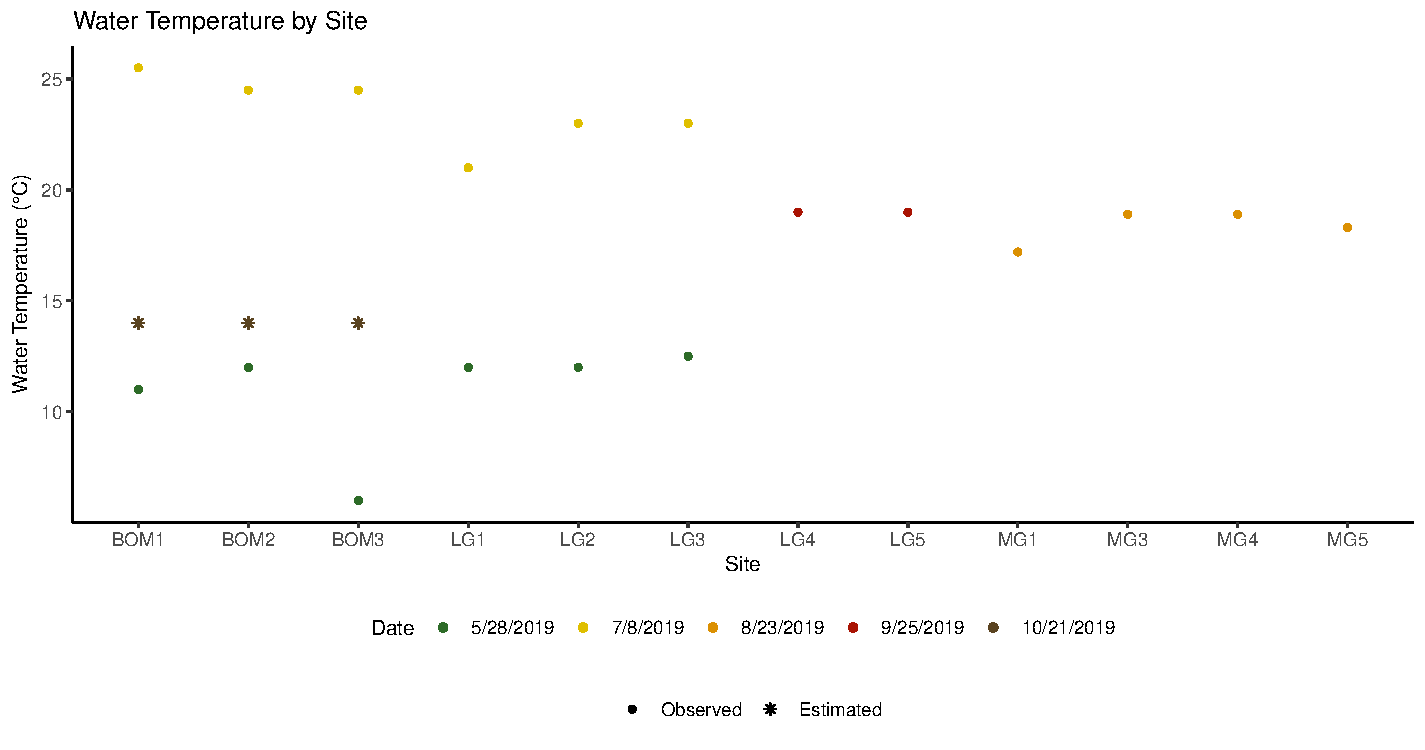
\includegraphics[width=\maxwidth]{figure/eDNA_visualization_temp-1} 

}



\end{knitrout}
\caption{A plot of the water temperatures by site, colored by the date on which the sample was taken. The estimated water temperatures are denoted with stars.}
\label{fig:eDNA_temp}
\end{figure}

\section{Methods}

\subsection{Bayesian Modeling Background}

In Bayesian statistics, inferences are based on the posterior distributions of the unknown parameters. The posterior distribution is a function of the likelihood of the observed data given a sampling model and some prior belief about the unknown parameters. Let $p(\bm{y}|\bm{\theta})$ denote the likelihood for some sampling model, and $p(\bm{\theta})$ denote the prior distribution on the unknown parameters $\bm{\theta}$. Then, using Bayes' rule, the posterior distribution, $p(\bm{\theta}|\bm{y})$, is: 

$$p(\bm{\theta}|\bm{y}) = \frac{p(\bm{y}|\bm{\theta})p(\bm{\theta})}{\int_\Theta p(\bm{y}|\bm{\theta})p(\bm{\theta})}$$

\noindent If the resulting posterior distribution is of the same distributional family as the prior distribution for the unknown parameter, then the prior is said to be conjugate for the sampling model. For example, if the observed data are $n$ independent binomial trails, with some unknown probability of success, $\theta$, and a beta prior distribution is used for $\theta$, it can be shown that the resulting posterior distribution is also a beta distribution. The complete model definition is: 

$$
\begin{aligned}
p(y_1, ..., y_n|\theta) &\sim binomial(n, \theta)\\
p(\theta) &\sim beta(\alpha, \beta)
\end{aligned}
$$

\noindent Using this, it can be shown that, 

$$p(\theta|y_1, ..., y_n) \sim beta \bigg( \sum_{i = 1}^n y_i + \alpha, n - \sum_{i = 1}^n y_i + \beta \bigg)$$

\noindent Therefore, since the prior distribution and the posterior distribution are of the same distributional family, then the beta prior is conjugate for the binomial sampling model.

However, the resulting posterior distribution is not always a named statistical distribution. In these situations, it is impossible to sample directly from the posterior distribution, but iterative sampling mechanisms can be used to approximate the unknown posterior distribution in order to make inferences. 

\subsubsection{Gibbs Sampler}

The most efficient iterative sampling technique available is the Gibbs sampler. In order to draw samples from an approximation of the joint posterior distribution using a Gibbs sampler, the full conditional posterior distribution of each of the unknown parameters must have a closed-form solution. The full conditional posterior distribution of a parameter is the distribution of that parameter, conditional on all other unknown parameters, the data, and the prior distributions. Once a full conditional posterior distribution is calculated for each unknown parameter, the iterative sampling can proceed in the following manner. 

\begin{mdframed}
\textit{Gibbs Sampler} \\
Let $\bm{\theta} = \{\theta_1, ..., \theta_p\}$ denote the vector of unknown parameters and $p(\theta_i|.)$ denote the full conditional distribution of $\theta_i$. The Gibbs Sampler generates the $s^{th}$ iteration as follows:
\begin{enumerate}
\item Sample $\theta_1^{(s)} \sim p(\theta_1|\theta_2^{(s-1)}, \theta_3^{(s-1)}, \dots, \theta_p^{(s-1)}, y_1, \dots, y_n)$. 
\item Sample $\theta_2^{(s)} \sim p(\theta_2|\theta_1^{(s)}, \theta_3^{(s-1)}, \dots, \theta_p^{(s-1)}, y_1, \dots, y_n)$.\\	
$\vdots$ \\[-14mm]
\item[$p$.] Sample $\theta_p^{(s)} \sim p(\theta_p|\theta_1^{(s)}, \theta_2^{(s)}, \dots, \theta_{p-1}^{(s)}, y_1, \dots , y_n)$. 
\end{enumerate}
\end{mdframed}

\noindent This process generates a dependent sequence of $\bm{\theta}$ vectors for each iteration, which together, converge to the joint posterior distribution, $p(\bm{\theta}|\bm{y})$. The Gibbs sampler is a basic Markov Chain Monte Carlo (MCMC) algorithm, where the current state only depends on the previous state, and additionally, the results should not depend on the starting values of $\bm{\theta}^{(0)}$.

One common use of a Gibbs sampler is for a normal sampling with unknown mean and variance. With this sampling model, a normal prior on the mean term and an inverse-gamma prior on the variance term enable the use of a Gibbs sampler to approximate the joint posterior distribution. However, in some cases, such as generalized linear models, semi-conjugate priors or closed-form solutions for the full conditional distributions are not available, and in those cases a Gibbs sampler cannot be used to sample from the joint posterior distribution of the unknown parameters. 

\subsubsection{Metropolis-Hastings Algorithm}

In cases that do not permit the use of a Gibbs sampler, a Metropolis-Hastings algorithm is often used to sample from the target distribution. Unlike a Gibbs sampler, a Metropolis-Hastings algorithm requires tuning, but proceeds in the following manner. 

\begin{mdframed}
\textit{Metropolis-Hastings Algorithm} \\
Let $\bm{\theta}^{(s)}$ be the current set of parameter estimates, $\bm{\theta}^*$ denote a new proposed set of parameters, and $J(\bm{\theta}^*|\bm{\theta}^{(s)})$ denote the proposal distribution, which is usually a random walk distribution. For example, $J(\bm{\theta}^*|\bm{\theta}^{(s)}) \sim MVN(\bm{\theta}^{(s)}, \gamma^2 \bm{I}_p)$ where $p$ is the number of unknown parameters, and $\gamma$ is thought of as the step size, or the average distance the proposed set of parameters falls from the current set. To complete an iteration: 
\begin{enumerate}
\item Sample $\bm{\theta}^*|\bm{\theta}^{(s)} \sim J(\bm{\theta}^*|\bm{\theta}^{(s)})$. 
\item Calculate the acceptance ratio $r = \frac{p(y|\bm{\theta}^*)p(\bm{\theta}^*)}{p(y|\bm{\theta}^{(s)})p(\bm{\theta}^{(s)})}$. 
\item Set $\bm{\theta}^{(s+1)}$:
\begin{itemize}
\item[-] If $r \geq 1$ then the proposed set, $\bm{\theta}^*$, is more attractive than the current set, $\bm{\theta}^{(s)}$, so $\bm{\theta}^{(s+1)} =   \bm{\theta}^*$. 
\item[-] If $r < 1$ then the proposed set, $\bm{\theta}^*$, is less attractive than the current set, $\bm{\theta}^{(s)}$, however the relative frequency of samples of $\bm{\theta}^*$ to $\bm{\theta}^{(s)}$ should be $r$, so with probability $r$, $\bm{\theta}^{(s+1)} = \bm{\theta}^*$.
\end{itemize}
\end{enumerate}
\end{mdframed}
  
\noindent The Metropolis algorithm is a generalization of the Metropolis-Hastings algorithm in which the proposal distribution is symmetric, meaning that $J(\bm{\theta}^*|\bm{\theta}^{(s)}) = J(\bm{\theta}^{(s)}|\bm{\theta}^*)$. The step size portion of the algorithm requires tuning and trace plots or other convergence tools should be used to ensure that the algorithm has efficiently explored the entire parameter space and converged to the true joint posterior distribution. 

\subsubsection{Bayesian Hierarchical Modeling}

Oftentimes data is collected in a hierarchical structure, that is data with a multilevel structure, such as students within classes, or sampling sites within a larger area of interest. For example, with two levels, the responses are independent observations from group $j$ and follow some distribution with unknown parameter $\theta_j$, meaning that $y_{1, j}, \dots, y_{n_j, j}|\theta_j \sim p(y|\theta_j)$; but the unknown parameters in each group are related to each other, such that they are independent samples from some distribution with parameter $\phi$, such that $\theta_1, \dots, \theta_m|\phi \sim p(\theta|\phi)$. With this representation, $p(y|\theta)$ is the variability among measurements within a group, and $p(\theta|\phi)$ is the sampling variability across groups. In order to completely specify the model, a prior distribution, $\phi \sim p(\psi)$, is needed for $\phi$. These models can be adapted to include covariates at each level, or to describe a more complicated structure with more levels. 

\subsection{Occupancy Models}

In ecological studies, there are several different state variables which may be of interest: abundance, vital rates, and occupancy are a few examples. Both mark-recapture and occupancy studies can be used to learn about the previously mentioned state variables, but there are advantages and limitations with each study type. In general, mark-recapture surveys are studies where individuals are capture or observed, given a unique mark, their identities recorded, and finally released; on subsequent occasions, both marked and unmarked individuals are captured, their identities recorded, unmarked individuals are marked, and they are all released. From this, capture histories, or encounter histories (typically a series of 0's and 1's) are recorded for each individual that is captured over the course of the study. There are several variations of mark-recapture studies, in which apparent survival, abundance, or both can be estimated depending on the study design. However, mark-recapture methods cannot be used when individuals of a species cannot be marked or uniquely identified. In this scenario, occupancy of a particular species can be recorded at each occasion. Occupancy methods are useful when studying a species over a large spatial scale for many years, particularly when the sampling sites are large relative to the species of interest. Though there is a loss in information about individuals of a species when occupancy studies are used, sometimes researchers are interested in the range of a species or the spread of invasion and therefore occupancy is the state variable of interest, and occupancy studies are most appropriate. Occupancy surveys are often used to track the mitigation efforts or spread of invasive species, but are plagued with imperfect detection probabilities. 

Occupancy models are a way to move past logistic regression for occupancy data in order to account for imperfect detection of the target species. However, multiple samples per site must be taken in order to learn about detection probabilities. For example, suppose five samples are taken from a site and two return a positive result, indicating that the species is present at the site, but the species was missed in three of the five samples, which provides information about the detectability of the species. There are several different types of occupancy models, but the traditional model is defined as follows. At the site level, $Z_i$ is defined as the presence ($Z_i = 1$) or absence ($Z_i = 0$) of the target species at the $i^{th}$ site ($i = 1, \dots, M$). Then, $Z_i \sim Bernoulli(\psi_i)$, where $\psi_i$ denotes the probability that the target species occupies the $i^{th}$ site. At the sample level, $Y_{ij}$ is defined as whether the target species is detected or not in the $j^{th}$ replicate at the $i^{th}$ site ($j = 1, \dots, J_{i}$). It follows that, $Y_{ij}|z_{ij} \sim Bernoulli(z_{i}p_{ij})$, where $z_i$ is the latent occupancy state for the $i^{th}$ site and $p_{ij}$ denotes the probability that the target species is detected on the $j^{th}$ survey, given the species occupies site $i$. Figure \ref{fig:ssocc} illustrates the structure of a traditional occupancy study, where each sample results in a binary response. 

\begin{figure}[]
	\centering
	
\includegraphics[scale = 0.7]{images/ssocc}
	\caption{A diagram displaying the structure of a traditional occupancy study.}
	\label{fig:ssocc}
\end{figure}

\noindent One assumption of occupancy models is that there is no unmodeled heterogeneity in the occupancy probabilities, or the detection probabilities, therefore covariates can be included at the site and sample levels. At the site level, $\bm{x}_i$ are the site specific covariates and $\bm{\beta}$ is the corresponding vector of regression parameters for $\psi_i$. At the sample level, $\bm{w}_{ij}$ are the sample specific covariates and $\bm{\alpha}$ is the corresponding vector of regression parameters for $p_{ij}$. It is also assumed that the sites are closed to changes in occupancy, so a site that is occupied at the beginning of the study should remain occupied throughout; if an occupancy study takes place over many years, there are models to account for the potential changes in occupancy status at the sites. Another assumption of these models is that the species is not misidentified, however, there are models that can account for false negative and false positive detections. The final assumption of these models is that the detection of the species is independent across sites. Violations of these assumptions can result in biased estimates of the occpuancy and detection probabilities. 

\subsubsection{Multi-scale Occupancy Models}

For more illusive species, the samples from each site are split into sub-samples, or replicates, and analyzed on a smaller scale. This introduces a hierarchical structure in the data creating dependencies which need to be accounted for \cite{MacKenzie}. One modeling approach to these types of data is the hierarchical latent state multi-scale occupancy model defined by Dorazio and Erickson which accounts for false negatives at the site, sample, and replicate levels \cite{Dorazio_Erickson}. The model is defined similarly to the traditional occupancy model described above, with an additional replicate level, the notation is as follows. At the site level, $Z_i$ is defined as the presence ($Z_i = 1$) or absence ($Z_i = 0$) of the target species at the $i^{th}$ site ($i = 1, \dots, M$). Then, $Z_i \sim Bernoulli(\psi_i)$, where $\psi_i$ denotes the probability that the target species occupies the $i^{th}$ site. At the sample level, $A_{ij}$ is defined as the presence or absence of the target species in the $j^{th}$ sample from the $i^{th}$ site ($j = 1, \dots, J_i$). Then, $A_{ij}|z_i \sim Bernoulli(z_i\theta_{ij})$, where $z_i$ is the latent occupancy state for the $i^{th}$ site, and $\theta_{ij}$ is the conditional probability that the target species is present in the $j^{th}$ sample from the $i^{th}$ site, given the target species is present at the site. At the replicate level, $Y_{ijk}$ is defined as whether the target species is detected or not in the $k^{th}$ replicate of the $j^{th}$ sample collected at the $i^{th}$ site ($k = 1, \dots, K_{ij}$). It follows that, $Y_{ijk}|a_{ij} \sim Bernoulli(a_{ij}p_{ijk})$, where $a_{ij}$ is the latent occupancy state for sample $j$ from site $i$, and $p_{ijk}$ is the conditional the probability that the target species is detected in the $k^{th}$ replicate of the $j^{th}$ sample collected at the $i^{th}$ site, given the target species is present in that sample. If $p_{ijk}$ does not differ among the replicates and the replicates are statistically independent, the replicate level can be simplified in the following manner: $Y_{ij}|a_{ij} \sim binomial(K_{ij}, a_{ij}p_{ij})$, where $Y_{ij} = \sum_{k = 1}^{K_{ij}}Y_{ijk}$, and $p_{ij}$ is the conditional probability of detection in each replicate of the $j^{th}$ sample collected at the $i^{th}$ location, given that the target species is present in that sample. Similiarly to above, an assumption of these models is that there is no unmodeled heterogeneity in the detection and occupancy probabilities, so covariates can be included in each level of the model to account for differences between individual sites, samples, or replicates; the notation for the covariates and corresponding regression parameters for the multi-scale occupancy model are as follows. At the site level, $\bm{x}_i$ are the site specific covariates and $\bm{\beta}$ is the corresponding vector of regression parameters for $\psi_i$. At the sample level, $\bm{w}_{ij}$ are the sample specific covariates and $\bm{\alpha}$ is the corresponding vector of regression parameters for $\theta_{ij}$. At the replication level, where there are no replicate level covariates, $\bm{v}_{ij}$ are the sample specific covariates and $\bm{\delta}$ is the corresponding vector of regression parameters for $p_{ij}$. Site specific covariates can be included for $\theta_{ij}$ and $p_{ij}$. The remaning assumptions from traditional occupancy models, described above, hold for multi-scale occupancy models as well.  

\subsection{Implementation}

There are several options for fitting occupancy models; the \texttt{R} package used for this analysis as well as some alternative methods for fitting occupancy models are described below. 

\subsubsection{\texttt{msocc} package}

\hl{\textit{get rid of this subsection?}}

The multi-scale occupancy model described above \cite{Dorazio_Erickson} can be easily fit in a Bayesian framework with the \texttt{msocc} package \cite{Stratton}. This package implements the P\'{o}lya Gamma data augmentation strategy described by Polson et. al (2013) to enable the use of a Gibbs Sampler in order to speed up the computation and avoid the tuning necessary for a Metropolis Algorithm. The model is specified in a familiar way to users of \texttt{R} at each level of the hierarchy in the model fitting function \texttt{msocc\_mod()}. To make the package more computationally efficient, there is an option to use the Beta-Binomial sampler when possible. Built into the package are posterior summary tools (\texttt{posterior\_summary()}) and a function for generating credible interval plots (\texttt{cred\_plot()}) at all levels of the hierarchy. 

\subsubsection{*implementation for traditional occupancy model*}



\subsubsection{Alternative Options}

There are several alternative options for fitting occupancy models. For example, the \texttt{eNDAoccupancy} \cite{Dorazio_Erickson} package fits the Bayesian multi-scale occupancy model defined above using a Metropolis-Hastings algorithm, which is less efficient and requires tuning. These models can also be written in \texttt{STAN} or \texttt{JAGS} and run in \texttt{R} using the packages \texttt{rstan} \cite{rstan} and \texttt{rjags} \cite{rjags} respectively, but again these methods are less computationally efficient than the methods described above. There are various frequentist methods for fitting occupancy models as well.  A commonly used \texttt{R} package for fitting frequentist occupancy models is \texttt{unmarked} \cite{unmarked}. Ecologists often utilize Program MARK, or access its functionalities through the \textt{R} package \texttt{RMark} \cite{RMark} to fit occupancy models, and other various models popular in ecology.

\section{Analysis}

\hl{\textit{A paragraph about the motivation to analyze the data this way, traditional occupancy model framework with the threshold }}











\begin{knitrout}
\definecolor{shadecolor}{rgb}{0.969, 0.969, 0.969}\color{fgcolor}\begin{kframe}
\begin{alltt}
\hlcom{# format data for use in PGocc4 function}
\hlcom{## number of samples per sites}
\hlstd{J} \hlkwb{<-} \hlkwd{rep}\hlstd{(}\hlnum{0}\hlstd{, M)}

\hlkwa{for}\hlstd{(j} \hlkwa{in} \hlnum{1}\hlopt{:}\hlkwd{length}\hlstd{(J))\{}
  \hlkwa{for}\hlstd{(i} \hlkwa{in} \hlnum{1}\hlopt{:}\hlkwd{nrow}\hlstd{(eDNA))\{}
    \hlkwa{if}\hlstd{(eDNA}\hlopt{$}\hlstd{Site[i]} \hlopt{==} \hlstd{Site.names[j])\{}
      \hlstd{J[j]} \hlkwb{<-} \hlstd{J[j]} \hlopt{+} \hlnum{1}
    \hlstd{\}}
  \hlstd{\}}
\hlstd{\}}


\hlcom{## number the from each site 1:J[i]}
\hlstd{samp} \hlkwb{<-} \hlkwd{matrix}\hlstd{(}\hlnum{NA}\hlstd{,} \hlkwc{nrow} \hlstd{= M,} \hlkwc{ncol} \hlstd{=} \hlkwd{max}\hlstd{(J))}

\hlkwa{for}\hlstd{(i} \hlkwa{in} \hlnum{1}\hlopt{:}\hlstd{M)\{}
  \hlkwa{if}\hlstd{(J[i]} \hlopt{==} \hlkwd{ncol}\hlstd{(samp))\{}
    \hlstd{samp[i, ]} \hlkwb{<-} \hlkwd{seq}\hlstd{(}\hlnum{1}\hlopt{:}\hlstd{J[i])}
  \hlstd{\}} \hlkwa{else} \hlstd{\{}
    \hlstd{samp[i,} \hlnum{1}\hlopt{:}\hlstd{J[i]]} \hlkwb{<-} \hlkwd{seq}\hlstd{(}\hlnum{1}\hlopt{:}\hlstd{J[i])}
  \hlstd{\}}
\hlstd{\}}

\hlstd{samp} \hlkwb{<-} \hlkwd{na.omit}\hlstd{(}\hlkwd{as.vector}\hlstd{(}\hlkwd{t}\hlstd{(samp)))}


\hlcom{## detection/non-detection matrix}
\hlstd{y} \hlkwb{<-} \hlkwd{matrix}\hlstd{(}\hlnum{NA}\hlstd{,} \hlkwc{nrow} \hlstd{= M,} \hlkwc{ncol} \hlstd{=} \hlkwd{max}\hlstd{(J))}

\hlkwa{for}\hlstd{(i} \hlkwa{in} \hlnum{1}\hlopt{:}\hlstd{M)\{}
  \hlkwa{for}\hlstd{(k} \hlkwa{in} \hlnum{1}\hlopt{:}\hlkwd{nrow}\hlstd{(eDNA))\{}
    \hlkwa{if}\hlstd{(eDNA}\hlopt{$}\hlstd{Site[k]} \hlopt{==} \hlstd{Site.names[i]} \hlopt{&} \hlstd{eDNA}\hlopt{$}\hlstd{Detect3[k]} \hlopt{==} \hlnum{1}\hlstd{)\{}
      \hlstd{y[i, samp[k]]} \hlkwb{<-} \hlnum{1}
    \hlstd{\}} \hlkwa{else if}\hlstd{(eDNA}\hlopt{$}\hlstd{Site[k]} \hlopt{==} \hlstd{Site.names[i]} \hlopt{&} \hlstd{eDNA}\hlopt{$}\hlstd{Detect3[k]} \hlopt{==} \hlnum{0}\hlstd{)\{}
      \hlstd{y[i, samp[k]]} \hlkwb{<-} \hlnum{0}
      \hlstd{\}}
  \hlstd{\}}
\hlstd{\}}

\hlstd{y} \hlkwb{<-} \hlkwd{matrix}\hlstd{(}\hlkwd{as.integer}\hlstd{(y),} \hlkwc{nrow} \hlstd{= M,} \hlkwc{ncol} \hlstd{=} \hlkwd{max}\hlstd{(J))}


\hlcom{## site level covariates}
\hlstd{avg.water.temp} \hlkwb{<-} \hlstd{eDNA} \hlopt
  \hlkwd{group_by}\hlstd{(Site)} \hlopt
  \hlkwd{summarise}\hlstd{(}\hlkwd{mean}\hlstd{(Water.Temp))}

\hlstd{X} \hlkwb{<-} \hlkwd{data.frame}\hlstd{(Site.names)}
\hlkwd{names}\hlstd{(X)} \hlkwb{<-} \hlstr{"site"}
\hlstd{X[,} \hlnum{2}\hlstd{]} \hlkwb{<-} \hlstd{X}\hlopt{$}\hlstd{site} \hlopt
  \hlkwd{as.character}\hlstd{()} \hlopt
  \hlkwd{removeNumbers}\hlstd{()} \hlopt
  \hlkwd{factor}\hlstd{()}
\hlstd{X} \hlkwb{<-} \hlkwd{cbind}\hlstd{(X, avg.water.temp[,} \hlnum{2}\hlstd{])}

\hlstd{X} \hlkwb{<-} \hlkwd{as.matrix}\hlstd{(X)}

\hlkwd{colnames}\hlstd{(X)[}\hlnum{2}\hlopt{:}\hlnum{3}\hlstd{]} \hlkwb{<-} \hlkwd{c}\hlstd{(}\hlstr{"lake"}\hlstd{,} \hlstr{"avg.water.temp"}\hlstd{)}


\hlcom{## sample level covariates}
\hlcom{### water temperature}
\hlstd{W1} \hlkwb{<-} \hlkwd{matrix}\hlstd{(}\hlnum{NA}\hlstd{,} \hlkwc{nrow} \hlstd{= M,} \hlkwc{ncol} \hlstd{=} \hlkwd{max}\hlstd{(J))}

\hlkwa{for}\hlstd{(i} \hlkwa{in} \hlnum{1}\hlopt{:}\hlstd{M)\{}
  \hlkwa{if}\hlstd{(J[i]} \hlopt{==} \hlkwd{ncol}\hlstd{(W1))\{}
    \hlstd{W1[i, ]} \hlkwb{<-} \hlstd{eDNA}\hlopt{$}\hlstd{Water.Temp[eDNA}\hlopt{$}\hlstd{Site} \hlopt{==} \hlstd{Site.names[i]]}
  \hlstd{\}} \hlkwa{else} \hlstd{\{}
    \hlstd{W1[i,} \hlnum{1}\hlopt{:}\hlstd{J[i]]} \hlkwb{<-} \hlstd{eDNA}\hlopt{$}\hlstd{Water.Temp[eDNA}\hlopt{$}\hlstd{Site} \hlopt{==} \hlstd{Site.names[i]]}
    \hlstd{\}}
\hlstd{\}}

\hlcom{### date}
\hlstd{W2} \hlkwb{<-} \hlkwd{data.frame}\hlstd{(}\hlkwd{matrix}\hlstd{(}\hlnum{NA}\hlstd{,} \hlkwc{nrow} \hlstd{= M,} \hlkwc{ncol} \hlstd{=} \hlkwd{max}\hlstd{(J)))}

\hlkwa{for}\hlstd{(i} \hlkwa{in} \hlnum{1}\hlopt{:}\hlstd{M)\{}
  \hlkwa{if}\hlstd{(J[i]} \hlopt{==} \hlkwd{ncol}\hlstd{(W2))\{}
    \hlstd{W2[i, ]} \hlkwb{<-} \hlstd{eDNA}\hlopt{$}\hlstd{Date.Collected[eDNA}\hlopt{$}\hlstd{Site} \hlopt{==} \hlstd{Site.names[i]]}
  \hlstd{\}} \hlkwa{else} \hlstd{\{}
    \hlstd{W2[i,} \hlnum{1}\hlopt{:}\hlstd{J[i]]} \hlkwb{<-} \hlstd{eDNA}\hlopt{$}\hlstd{Date.Collected[eDNA}\hlopt{$}\hlstd{Site} \hlopt{==} \hlstd{Site.names[i]]}
    \hlstd{\}}
\hlstd{\}}

\hlstd{W2} \hlkwb{<-} \hlkwd{as.matrix}\hlstd{(W2)}

\hlcom{### site }
\hlstd{W3} \hlkwb{<-} \hlkwd{data.frame}\hlstd{(}\hlkwd{matrix}\hlstd{(}\hlnum{NA}\hlstd{,} \hlkwc{nrow} \hlstd{= M,} \hlkwc{ncol} \hlstd{=} \hlkwd{max}\hlstd{(J)))}

\hlkwa{for}\hlstd{(i} \hlkwa{in} \hlnum{1}\hlopt{:}\hlstd{M)\{}
  \hlkwa{if}\hlstd{(J[i]} \hlopt{==} \hlkwd{ncol}\hlstd{(W3))\{}
    \hlstd{W3[i, ]} \hlkwb{<-} \hlstd{eDNA}\hlopt{$}\hlstd{Site[eDNA}\hlopt{$}\hlstd{Site} \hlopt{==} \hlstd{Site.names[i]]}
  \hlstd{\}} \hlkwa{else} \hlstd{\{}
    \hlstd{W3[i,} \hlnum{1}\hlopt{:}\hlstd{J[i]]} \hlkwb{<-} \hlstd{eDNA}\hlopt{$}\hlstd{Site[eDNA}\hlopt{$}\hlstd{Site} \hlopt{==} \hlstd{Site.names[i]]}
    \hlstd{\}}
\hlstd{\}}

\hlstd{W3} \hlkwb{<-} \hlkwd{as.matrix}\hlstd{(W3)}

\hlstd{W} \hlkwb{<-} \hlkwd{list}\hlstd{(}\hlkwc{W1} \hlstd{= W1,} \hlkwc{W2} \hlstd{= W2,} \hlkwc{W3} \hlstd{= W3)}


\hlcom{# merge for use in PGocc4}
\hlstd{data} \hlkwb{<-} \hlkwd{vb_Designs}\hlstd{(}\hlkwc{W} \hlstd{= W,} \hlkwc{X} \hlstd{= X,} \hlkwc{y} \hlstd{= y)}
\end{alltt}
\end{kframe}
\end{knitrout}

\begin{knitrout}
\definecolor{shadecolor}{rgb}{0.969, 0.969, 0.969}\color{fgcolor}\begin{kframe}
\begin{alltt}
\hlstd{post_summary} \hlkwb{<-} \hlkwa{function}\hlstd{(}\hlkwc{parameter.matrix}\hlstd{,} \hlkwc{param}\hlstd{,} \hlkwc{plot.options} \hlstd{=} \hlkwa{NULL}\hlstd{,} \hlkwc{plot} \hlstd{= T)\{}
  \hlstd{mean} \hlkwb{<-} \hlkwd{apply}\hlstd{(parameter.matrix,} \hlnum{1}\hlstd{, mean)}
  \hlstd{median} \hlkwb{<-} \hlkwd{apply}\hlstd{(parameter.matrix,} \hlnum{1}\hlstd{, median)}
  \hlstd{lwr} \hlkwb{<-} \hlkwd{apply}\hlstd{(parameter.matrix,} \hlnum{1}\hlstd{, quantile,} \hlkwc{probs} \hlstd{=} \hlnum{0.025}\hlstd{)}
  \hlstd{upr} \hlkwb{<-} \hlkwd{apply}\hlstd{(parameter.matrix,} \hlnum{1}\hlstd{, quantile,} \hlkwc{probs} \hlstd{=} \hlnum{0.975}\hlstd{)}
  \hlstd{out} \hlkwb{<-} \hlkwd{cbind}\hlstd{(}\hlstr{"mean"} \hlstd{= mean,} \hlstr{"median"} \hlstd{= median,} \hlstr{"2.5%"} \hlstd{= lwr ,} \hlstr{"97.5%"} \hlstd{= upr)}
  \hlkwa{if}\hlstd{(}\hlkwd{missing}\hlstd{(param))\{}
    \hlstd{out} \hlkwb{<-} \hlstd{out}
  \hlstd{\}} \hlkwa{else if}\hlstd{(param} \hlopt{==} \hlstr{"psi"}\hlstd{)\{}
    \hlstd{out} \hlkwb{<-} \hlkwd{cbind.data.frame}\hlstd{(out,} \hlkwc{rownames} \hlstd{= Site.names)}
  \hlstd{\}} \hlkwa{else if}\hlstd{(param} \hlopt{==} \hlstr{"p"}\hlstd{)\{}
    \hlstd{out} \hlkwb{<-} \hlkwd{cbind.data.frame}\hlstd{(}\hlkwc{Site} \hlstd{= eDNA}\hlopt{$}\hlstd{Site,} \hlkwc{Sample} \hlstd{= samp, out)}
  \hlstd{\}} \hlkwa{else if}\hlstd{(param} \hlopt{==} \hlstr{"alpha"}\hlstd{)\{}
    \hlkwd{rownames}\hlstd{(out)} \hlkwb{<-} \hlkwd{paste}\hlstd{(}\hlstr{"alpha"}\hlstd{,} \hlnum{0}\hlopt{:}\hlstd{(}\hlkwd{nrow}\hlstd{(out)} \hlopt{-} \hlnum{1}\hlstd{))}
  \hlstd{\}} \hlkwa{else if}\hlstd{(param} \hlopt{==} \hlstr{"beta"}\hlstd{)\{}
    \hlkwd{rownames}\hlstd{(out)} \hlkwb{<-} \hlkwd{paste}\hlstd{(}\hlstr{"beta"}\hlstd{,} \hlnum{0}\hlopt{:}\hlstd{(}\hlkwd{nrow}\hlstd{(out)} \hlopt{-} \hlnum{1}\hlstd{))}
  \hlstd{\}}
  \hlkwa{if}\hlstd{(plot} \hlopt{==} \hlstd{T)\{}
    \hlkwa{for}\hlstd{(i} \hlkwa{in} \hlnum{1}\hlopt{:}\hlkwd{nrow}\hlstd{(parameter.matrix))\{}
      \hlstd{df} \hlkwb{<-} \hlkwd{data.frame}\hlstd{(parameter.matrix[i, ])}
      \hlstd{tr.plot} \hlkwb{<-} \hlkwd{ggplot}\hlstd{(df,} \hlkwd{aes}\hlstd{(}\hlkwc{x} \hlstd{=} \hlnum{1}\hlopt{:}\hlkwd{ncol}\hlstd{(parameter.matrix),} \hlkwc{y} \hlstd{= parameter.matrix[i, ]))} \hlopt{+}
        \hlkwd{geom_path}\hlstd{()} \hlopt{+}
        \hlkwd{xlab}\hlstd{(}\hlstr{"Post Burn-in Iterations"}\hlstd{)} \hlopt{+}
        \hlkwd{ylab}\hlstd{(}\hlkwd{rownames}\hlstd{(out)[i])} \hlopt{+}
        \hlkwd{theme_bw}\hlstd{()} \hlopt{+}
          \hlkwd{theme}\hlstd{(}\hlkwc{title} \hlstd{=} \hlkwd{element_text}\hlstd{(}\hlkwc{size} \hlstd{=} \hlnum{10}\hlstd{),}
                \hlkwc{panel.border} \hlstd{=} \hlkwd{element_blank}\hlstd{(),}
                \hlkwc{panel.grid.major} \hlstd{=} \hlkwd{element_blank}\hlstd{(),}
                \hlkwc{panel.grid.minor} \hlstd{=} \hlkwd{element_blank}\hlstd{(),}
                \hlkwc{axis.line} \hlstd{=} \hlkwd{element_line}\hlstd{(}\hlkwc{colour} \hlstd{=} \hlstr{"black"}\hlstd{))}
      \hlkwa{if}\hlstd{(}\hlkwd{is.null}\hlstd{(plot.options))\{}
        \hlstd{tr.plot} \hlkwb{<-} \hlstd{tr.plot}
        \hlstd{\}} \hlkwa{else} \hlstd{\{}
          \hlstd{tr.plot} \hlkwb{<-} \hlstd{tr.plot} \hlopt{+} \hlstd{plot.options\}}
      \hlkwd{print}\hlstd{(tr.plot)}
    \hlstd{\}}
  \hlstd{\}}
  \hlkwd{return}\hlstd{(out)}
\hlstd{\}}
\end{alltt}
\end{kframe}
\end{knitrout}

\begin{knitrout}
\definecolor{shadecolor}{rgb}{0.969, 0.969, 0.969}\color{fgcolor}\begin{kframe}
\begin{alltt}
\hlstd{cred_plot} \hlkwb{<-} \hlkwa{function}\hlstd{(}\hlkwc{post_summary_out}\hlstd{,} \hlkwc{parameter}\hlstd{)\{}
  \hlstd{df} \hlkwb{<-} \hlkwd{data.frame}\hlstd{(post_summary_out)}
  \hlkwa{if}\hlstd{(}\hlkwd{nrow}\hlstd{(df)} \hlopt{==} \hlnum{12}\hlstd{)\{}
    \hlkwd{rownames}\hlstd{(df)} \hlkwb{<-} \hlstd{Site.names}
  \hlstd{\}}
  \hlkwa{if}\hlstd{(parameter} \hlopt{==} \hlstr{"psi"}\hlstd{)\{}
    \hlstd{cred.plot} \hlkwb{<-} \hlkwd{ggplot}\hlstd{(df,} \hlkwd{aes}\hlstd{(}\hlkwc{x} \hlstd{=} \hlkwd{rownames}\hlstd{(df),} \hlkwc{y} \hlstd{= mean))} \hlopt{+}
      \hlkwd{geom_point}\hlstd{()} \hlopt{+}
      \hlkwd{xlab}\hlstd{(}\hlstr{""}\hlstd{)} \hlopt{+}
      \hlkwd{geom_errorbar}\hlstd{(}\hlkwd{aes}\hlstd{(}\hlkwc{ymax} \hlstd{= X97.5.,} \hlkwc{ymin} \hlstd{= X2.5.),} \hlkwc{width} \hlstd{=} \hlnum{0}\hlstd{)} \hlopt{+}
      \hlkwd{theme_bw}\hlstd{()} \hlopt{+}
      \hlkwd{theme}\hlstd{(}\hlkwc{title} \hlstd{=} \hlkwd{element_text}\hlstd{(}\hlkwc{size} \hlstd{=} \hlnum{10}\hlstd{),}
            \hlkwc{panel.border} \hlstd{=} \hlkwd{element_blank}\hlstd{(),}
            \hlkwc{panel.grid.major} \hlstd{=} \hlkwd{element_blank}\hlstd{(),}
            \hlkwc{panel.grid.minor} \hlstd{=} \hlkwd{element_blank}\hlstd{(),}
            \hlkwc{axis.line} \hlstd{=} \hlkwd{element_line}\hlstd{(}\hlkwc{colour} \hlstd{=} \hlstr{"black"}\hlstd{),}
            \hlkwc{axis.text.x} \hlstd{=} \hlkwd{element_text}\hlstd{(}\hlkwc{angle} \hlstd{=} \hlnum{45}\hlstd{,} \hlkwc{hjust} \hlstd{=} \hlnum{1}\hlstd{))} \hlopt{+}
      \hlkwd{ylab}\hlstd{(}\hlkwd{expression}\hlstd{(}\hlkwd{paste}\hlstd{(}\hlstr{"Estimated "}\hlstd{, psi)))}
  \hlstd{\}} \hlkwa{else if}\hlstd{(parameter} \hlopt{==} \hlstr{"p"}\hlstd{)\{}
    \hlstd{cred.plot} \hlkwb{<-} \hlkwd{ggplot}\hlstd{(df,} \hlkwd{aes}\hlstd{(}\hlkwc{x} \hlstd{= eDNA}\hlopt{$}\hlstd{Date.Collected,} \hlkwc{y} \hlstd{= mean))} \hlopt{+}
      \hlkwd{geom_point}\hlstd{()} \hlopt{+}
      \hlkwd{xlab}\hlstd{(}\hlstr{""}\hlstd{)} \hlopt{+}
      \hlkwd{geom_errorbar}\hlstd{(}\hlkwd{aes}\hlstd{(}\hlkwc{ymax} \hlstd{= X97.5.,} \hlkwc{ymin} \hlstd{= X2.5.),} \hlkwc{width} \hlstd{=} \hlnum{0}\hlstd{)} \hlopt{+}
      \hlkwd{theme_bw}\hlstd{()} \hlopt{+}
      \hlkwd{theme}\hlstd{(}\hlkwc{title} \hlstd{=} \hlkwd{element_text}\hlstd{(}\hlkwc{size} \hlstd{=} \hlnum{10}\hlstd{),}
            \hlkwc{panel.border} \hlstd{=} \hlkwd{element_blank}\hlstd{(),}
            \hlkwc{panel.grid.major} \hlstd{=} \hlkwd{element_blank}\hlstd{(),}
            \hlkwc{panel.grid.minor} \hlstd{=} \hlkwd{element_blank}\hlstd{(),}
            \hlkwc{axis.line} \hlstd{=} \hlkwd{element_line}\hlstd{(}\hlkwc{colour} \hlstd{=} \hlstr{"black"}\hlstd{),}
            \hlkwc{axis.text.x} \hlstd{=} \hlkwd{element_text}\hlstd{(}\hlkwc{angle} \hlstd{=} \hlnum{45}\hlstd{,} \hlkwc{hjust} \hlstd{=} \hlnum{1}\hlstd{))} \hlopt{+}
      \hlkwd{ylab}\hlstd{(}\hlstr{"Estimated p"}\hlstd{)} \hlopt{+}
      \hlkwd{facet_wrap}\hlstd{(}\hlopt{~}\hlstd{Site)}
  \hlstd{\}}
  \hlkwd{print}\hlstd{(cred.plot)}
\hlstd{\}}
\end{alltt}
\end{kframe}
\end{knitrout}












\section{Results}

\subsection{Ecological Implications}

when analyzed at the droplet level, less confident about negative result

\subsection{Sampling Recommendations}

\section{Future Work}

arbitrary amplitude cutoff for choosing the droplets that are positive and negative

threshold for the number of positive droplets to be considered a positive sample 

what is a false positive and how does it bias the results 

discussion of droplet level and how multi-scale occupancy model can 

\section{Acknowledgements}

\nocite{*}

\newpage
\section{References}

\begingroup
\renewcommand{\section}[2]{}%
\begin{flushleft}
\bibliographystyle{apalike}
%\bibliographystyle{acm}
%\bibliographystyle{abbrvnat}
%\bibliographystyle{unsrtnat}
%\bibliographystyle{ACM-Reference-Format}
\bibliography{bibliography}
\end{flushleft}
\endgroup

\newpage
\section{Appendix - R Code}

\singlespacing

\begin{knitrout}
\definecolor{shadecolor}{rgb}{0.969, 0.969, 0.969}\color{fgcolor}\begin{kframe}
\begin{verbatim}
# packages used 
library(car)
library(dplyr)
library(tidyr)
library(dataRetrieval)
library(kableExtra)
library(ggplot2)
library(gridExtra)
library(tm)
library(readxl)
## library(devtools)
## devtools::install_github("StrattonCh/msocc")
library(msocc)
library(Rcppocc)



# load eDNA data
eDNA <- read.csv(
  "C:/Users/mwind/OneDrive/Writing Project_EXTRA/eDNA.csv")


# rename lakes
levels(eDNA$Lake) <- c("BOM", "LG", "MG")


# remove field blank samples
eDNA <- eDNA %>% 
  filter(Site != "tb")
eDNA$Site <- droplevels(eDNA$Site)


# reorder dates in chronological order
eDNA$Date.Collected <- factor(eDNA$Date.Collected,
                          levels = c("5/28/2019", 
                                     "7/8/2019", 
                                     "8/23/2019", 
                                     "9/25/2019",
                                     "10/21/2019"))


Site.names <- unique(eDNA$Site)

M <- length(Site.names)


lake <- eDNA$Site %>% 
  as.character() %>%
  removeNumbers() %>%
  factor()


# generate table of 10 sample rows of eDNA data
set.seed(03142020)
knitr::kable(some(eDNA), 'latex', booktabs = T, linesep = "",
             caption = "\\label{tab:eDNA_data}
             10 sample rows of the eDNA data.", 
             align = 'c', row.names = F, 
             col.names = c("Lake", "Site", "Sample", "Date", 
                           "Water Temperature", "Concentration", 
                           "Positive Droplets")) %>%
  kable_styling(latex_options = 
                  c("scale_down", "hold_position"))
\end{verbatim}
\end{kframe}
\end{knitrout}


\lstset{
	basicstyle=\ttfamily\scriptsize,
	columns = fullflexible,
	frame = single,
	breaklines = true,
	postbreak = \mbox{\textcolor{red}{$\hookrightarrow$}\space},
	keepspaces = TRUE,
}
%\begin{lstlisting}
%\end{lstlisting}
\end{document}
              
